% Created by tikzDevice version 0.12.6 on 2024-11-10 09:54:48
% !TEX encoding = UTF-8 Unicode
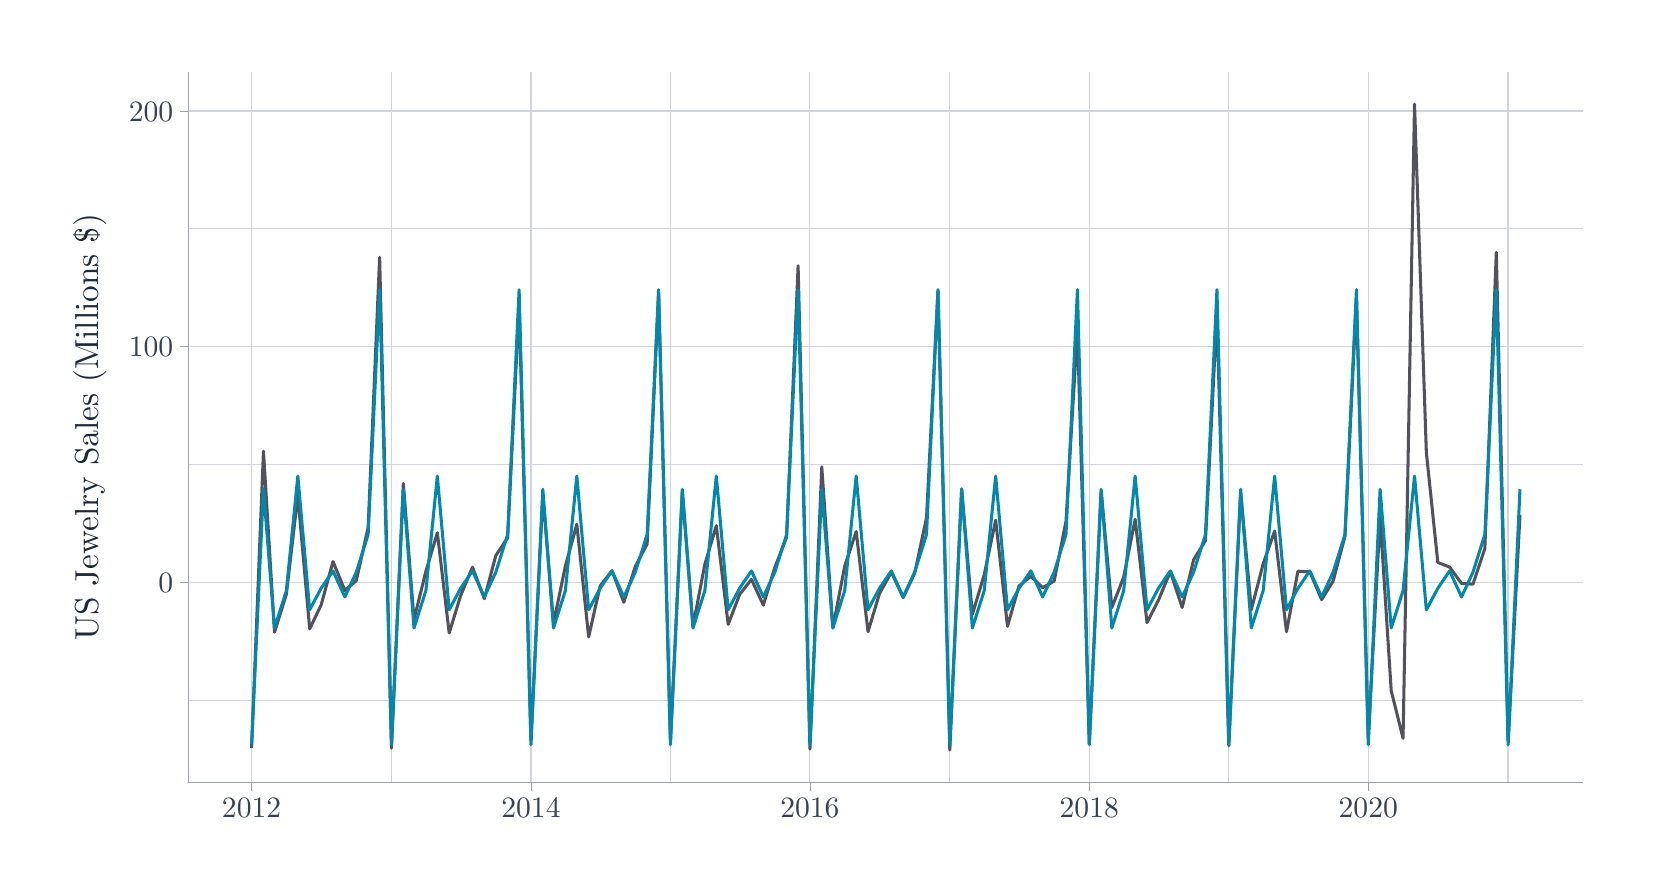
\begin{tikzpicture}[x=1pt,y=1pt]
\definecolor{fillColor}{RGB}{255,255,255}
\path[use as bounding box,fill=fillColor] (0,0) rectangle (578.16,303.53);
\begin{scope}
\path[clip] (  0.00,  0.00) rectangle (578.16,303.53);
\definecolor{drawColor}{RGB}{255,255,255}

\path[draw=drawColor,line width= 0.6pt,line join=round,line cap=round,fill=fillColor] (  0.00,  0.00) rectangle (578.16,303.53);
\end{scope}
\begin{scope}
\path[clip] ( 58.00, 30.82) rectangle (562.16,287.53);
\definecolor{drawColor}{RGB}{255,255,255}
\definecolor{fillColor}{RGB}{255,255,255}

\path[draw=drawColor,line width= 0.6pt,line join=round,line cap=round,fill=fillColor] ( 58.00, 30.82) rectangle (562.16,287.53);
\definecolor{drawColor}{RGB}{209,213,219}

\path[draw=drawColor,line width= 0.4pt,line join=round] ( 58.00, 60.46) --
	(562.16, 60.46);

\path[draw=drawColor,line width= 0.4pt,line join=round] ( 58.00,145.64) --
	(562.16,145.64);

\path[draw=drawColor,line width= 0.4pt,line join=round] ( 58.00,230.81) --
	(562.16,230.81);

\path[draw=drawColor,line width= 0.4pt,line join=round] (131.39, 30.82) --
	(131.39,287.53);

\path[draw=drawColor,line width= 0.4pt,line join=round] (232.26, 30.82) --
	(232.26,287.53);

\path[draw=drawColor,line width= 0.4pt,line join=round] (333.14, 30.82) --
	(333.14,287.53);

\path[draw=drawColor,line width= 0.4pt,line join=round] (434.02, 30.82) --
	(434.02,287.53);

\path[draw=drawColor,line width= 0.4pt,line join=round] (534.89, 30.82) --
	(534.89,287.53);

\path[draw=drawColor,line width= 0.4pt,line join=round] ( 58.00,103.05) --
	(562.16,103.05);

\path[draw=drawColor,line width= 0.4pt,line join=round] ( 58.00,188.22) --
	(562.16,188.22);

\path[draw=drawColor,line width= 0.4pt,line join=round] ( 58.00,273.40) --
	(562.16,273.40);

\path[draw=drawColor,line width= 0.4pt,line join=round] ( 80.91, 30.82) --
	( 80.91,287.53);

\path[draw=drawColor,line width= 0.4pt,line join=round] (181.86, 30.82) --
	(181.86,287.53);

\path[draw=drawColor,line width= 0.4pt,line join=round] (282.67, 30.82) --
	(282.67,287.53);

\path[draw=drawColor,line width= 0.4pt,line join=round] (383.61, 30.82) --
	(383.61,287.53);

\path[draw=drawColor,line width= 0.4pt,line join=round] (484.42, 30.82) --
	(484.42,287.53);
\definecolor{drawColor}{RGB}{82,82,91}

\path[draw=drawColor,line width= 1.1pt,line join=round] ( 80.91, 43.26) --
	( 85.20,150.49) --
	( 89.20, 85.08) --
	( 93.48, 98.79) --
	( 97.62,134.48) --
	(101.90, 86.27) --
	(106.05, 94.96) --
	(110.33,110.63) --
	(114.61,100.15) --
	(118.75,103.73) --
	(123.03,122.98) --
	(127.18,220.59) --
	(131.46, 43.17) --
	(135.74,138.82) --
	(139.60, 89.68) --
	(143.89,107.05) --
	(148.03,121.02) --
	(152.31, 84.82) --
	(156.45, 98.28) --
	(160.73,108.59) --
	(165.01, 97.17) --
	(169.16,112.76) --
	(173.44,119.23) --
	(177.58,203.21) --
	(181.86, 45.90) --
	(186.14,134.82) --
	(190.01, 88.31) --
	(194.29,108.93) --
	(198.43,124.09) --
	(202.71, 83.37) --
	(206.86,101.77) --
	(211.14,107.31) --
	(215.42, 95.89) --
	(219.56,108.84) --
	(223.84,116.93) --
	(227.98,207.47) --
	(232.26, 45.81) --
	(236.55,135.76) --
	(240.41, 87.21) --
	(244.69,109.61) --
	(248.84,123.58) --
	(253.12, 87.89) --
	(257.26, 98.71) --
	(261.54,104.16) --
	(265.82, 94.87) --
	(269.96,108.42) --
	(274.24,119.40) --
	(278.39,217.52) --
	(282.67, 42.83) --
	(286.95,144.78) --
	(290.95, 86.61) --
	(295.23,108.93) --
	(299.38,121.45) --
	(303.66, 85.25) --
	(307.80, 99.05) --
	(312.08,106.80) --
	(316.36, 97.60) --
	(320.51,106.37) --
	(324.79,126.39) --
	(328.93,208.32) --
	(333.21, 42.49) --
	(337.49,136.86) --
	(341.36, 91.47) --
	(345.64,105.86) --
	(349.78,125.54) --
	(354.06, 87.21) --
	(358.20,101.77) --
	(362.49,105.26) --
	(366.77,101.18) --
	(370.91,103.56) --
	(375.19,125.11) --
	(379.33,194.61) --
	(383.61, 44.71) --
	(387.89,136.10) --
	(391.76, 93.94) --
	(396.04,105.01) --
	(400.18,125.88) --
	(404.47, 88.57) --
	(408.61, 96.66) --
	(412.89,106.97) --
	(417.17, 94.02) --
	(421.31,111.23) --
	(425.59,118.21) --
	(429.74,200.32) --
	(434.02, 44.02) --
	(438.30,135.67) --
	(442.16, 93.17) --
	(446.45,109.86) --
	(450.59,121.62) --
	(454.87, 85.25) --
	(459.01,107.14) --
	(463.29,106.88) --
	(467.57, 96.83) --
	(471.72,103.56) --
	(476.00,119.74) --
	(480.14,205.34) --
	(484.42, 46.75) --
	(488.70,126.47) --
	(492.71, 63.96) --
	(496.99, 46.75) --
	(501.13,275.87) --
	(505.41,149.98) --
	(509.55,110.29) --
	(513.83,108.59) --
	(518.12,102.71) --
	(522.26,102.45) --
	(526.54,115.31) --
	(530.68,222.29) --
	(534.96, 45.47) --
	(539.24,127.49);
\definecolor{drawColor}{RGB}{1,136,172}

\path[draw=drawColor,line width= 1.1pt,line join=round] ( 80.91, 44.44) --
	( 85.20,136.73) --
	( 89.20, 86.60) --
	( 93.48,100.09) --
	( 97.62,141.50) --
	(101.90, 93.18) --
	(106.05,100.96) --
	(110.33,107.24) --
	(114.61, 97.83) --
	(118.75,106.77) --
	(123.03,120.37) --
	(127.18,208.85) --
	(131.46, 44.44) --
	(135.74,136.73) --
	(139.60, 86.60) --
	(143.89,100.09) --
	(148.03,141.50) --
	(152.31, 93.18) --
	(156.45,100.96) --
	(160.73,107.24) --
	(165.01, 97.83) --
	(169.16,106.77) --
	(173.44,120.37) --
	(177.58,208.85) --
	(181.86, 44.44) --
	(186.14,136.73) --
	(190.01, 86.60) --
	(194.29,100.09) --
	(198.43,141.50) --
	(202.71, 93.18) --
	(206.86,100.96) --
	(211.14,107.24) --
	(215.42, 97.83) --
	(219.56,106.77) --
	(223.84,120.37) --
	(227.98,208.85) --
	(232.26, 44.44) --
	(236.55,136.73) --
	(240.41, 86.60) --
	(244.69,100.09) --
	(248.84,141.50) --
	(253.12, 93.18) --
	(257.26,100.96) --
	(261.54,107.24) --
	(265.82, 97.83) --
	(269.96,106.77) --
	(274.24,120.37) --
	(278.39,208.85) --
	(282.67, 44.44) --
	(286.95,136.73) --
	(290.95, 86.60) --
	(295.23,100.09) --
	(299.38,141.50) --
	(303.66, 93.18) --
	(307.80,100.96) --
	(312.08,107.24) --
	(316.36, 97.83) --
	(320.51,106.77) --
	(324.79,120.37) --
	(328.93,208.85) --
	(333.21, 44.44) --
	(337.49,136.73) --
	(341.36, 86.60) --
	(345.64,100.09) --
	(349.78,141.50) --
	(354.06, 93.18) --
	(358.20,100.96) --
	(362.49,107.24) --
	(366.77, 97.83) --
	(370.91,106.77) --
	(375.19,120.37) --
	(379.33,208.85) --
	(383.61, 44.44) --
	(387.89,136.73) --
	(391.76, 86.60) --
	(396.04,100.09) --
	(400.18,141.50) --
	(404.47, 93.18) --
	(408.61,100.96) --
	(412.89,107.24) --
	(417.17, 97.83) --
	(421.31,106.77) --
	(425.59,120.37) --
	(429.74,208.85) --
	(434.02, 44.44) --
	(438.30,136.73) --
	(442.16, 86.60) --
	(446.45,100.09) --
	(450.59,141.50) --
	(454.87, 93.18) --
	(459.01,100.96) --
	(463.29,107.24) --
	(467.57, 97.83) --
	(471.72,106.77) --
	(476.00,120.37) --
	(480.14,208.85) --
	(484.42, 44.44) --
	(488.70,136.73) --
	(492.71, 86.60) --
	(496.99,100.09) --
	(501.13,141.50) --
	(505.41, 93.18) --
	(509.55,100.96) --
	(513.83,107.24) --
	(518.12, 97.83) --
	(522.26,106.77) --
	(526.54,120.37) --
	(530.68,208.85) --
	(534.96, 44.44) --
	(539.24,136.73);
\end{scope}
\begin{scope}
\path[clip] (  0.00,  0.00) rectangle (578.16,303.53);
\definecolor{drawColor}{RGB}{156,163,175}

\path[draw=drawColor,line width= 0.3pt,line join=round] ( 58.00, 30.82) --
	( 58.00,287.53);
\end{scope}
\begin{scope}
\path[clip] (  0.00,  0.00) rectangle (578.16,303.53);
\definecolor{drawColor}{RGB}{55,65,81}

\node[text=drawColor,anchor=base east,inner sep=0pt, outer sep=0pt, scale=  1.07] at ( 52.60, 99.38) {0};

\node[text=drawColor,anchor=base east,inner sep=0pt, outer sep=0pt, scale=  1.07] at ( 52.60,184.55) {100};

\node[text=drawColor,anchor=base east,inner sep=0pt, outer sep=0pt, scale=  1.07] at ( 52.60,269.72) {200};
\end{scope}
\begin{scope}
\path[clip] (  0.00,  0.00) rectangle (578.16,303.53);
\definecolor{drawColor}{RGB}{156,163,175}

\path[draw=drawColor,line width= 0.3pt,line join=round] ( 55.00,103.05) --
	( 58.00,103.05);

\path[draw=drawColor,line width= 0.3pt,line join=round] ( 55.00,188.22) --
	( 58.00,188.22);

\path[draw=drawColor,line width= 0.3pt,line join=round] ( 55.00,273.40) --
	( 58.00,273.40);
\end{scope}
\begin{scope}
\path[clip] (  0.00,  0.00) rectangle (578.16,303.53);
\definecolor{drawColor}{RGB}{156,163,175}

\path[draw=drawColor,line width= 0.3pt,line join=round] ( 58.00, 30.82) --
	(562.16, 30.82);
\end{scope}
\begin{scope}
\path[clip] (  0.00,  0.00) rectangle (578.16,303.53);
\definecolor{drawColor}{RGB}{156,163,175}

\path[draw=drawColor,line width= 0.3pt,line join=round] ( 80.91, 27.82) --
	( 80.91, 30.82);

\path[draw=drawColor,line width= 0.3pt,line join=round] (181.86, 27.82) --
	(181.86, 30.82);

\path[draw=drawColor,line width= 0.3pt,line join=round] (282.67, 27.82) --
	(282.67, 30.82);

\path[draw=drawColor,line width= 0.3pt,line join=round] (383.61, 27.82) --
	(383.61, 30.82);

\path[draw=drawColor,line width= 0.3pt,line join=round] (484.42, 27.82) --
	(484.42, 30.82);
\end{scope}
\begin{scope}
\path[clip] (  0.00,  0.00) rectangle (578.16,303.53);
\definecolor{drawColor}{RGB}{55,65,81}

\node[text=drawColor,anchor=base,inner sep=0pt, outer sep=0pt, scale=  1.07] at ( 80.91, 18.07) {2012};

\node[text=drawColor,anchor=base,inner sep=0pt, outer sep=0pt, scale=  1.07] at (181.86, 18.07) {2014};

\node[text=drawColor,anchor=base,inner sep=0pt, outer sep=0pt, scale=  1.07] at (282.67, 18.07) {2016};

\node[text=drawColor,anchor=base,inner sep=0pt, outer sep=0pt, scale=  1.07] at (383.61, 18.07) {2018};

\node[text=drawColor,anchor=base,inner sep=0pt, outer sep=0pt, scale=  1.07] at (484.42, 18.07) {2020};
\end{scope}
\begin{scope}
\path[clip] (  0.00,  0.00) rectangle (578.16,303.53);
\definecolor{drawColor}{RGB}{31,41,55}

\node[text=drawColor,rotate= 90.00,anchor=base,inner sep=0pt, outer sep=0pt, scale=  1.20] at ( 25.43,159.18) {US Jewelry Sales (Millions \$)};
\end{scope}
\end{tikzpicture}
